\documentclass[a4paper, twocolumn]{article}

\usepackage[a4paper, left=14.5mm, right=15mm, top=20mm, bottom=32mm]{geometry}
\usepackage[english]{babel}
\usepackage{graphicx}

\pagenumbering{arabic}
\bibliographystyle{}

\title{
	\LARGE{
		\textbf{
			Project Heirs Briefing
		}
	}
}

\author{
	Farhad Modaresi\footnote{B.Eng. in Electrical Engineering}
}
\date{July 12, 2021}
\begin{document}
\maketitle


\begin{abstract}
	This project aims to design a bench power supply to fill the hollow points in the rather disturbed Iranian market. High availability, durability of the product, targeting a wide range of users, selling accessories, modular design, low price tag, a road map for future development, and making the product open source would be among the factors that will help secure market share and profitability. The focus point however would be on the low profit margins of a primary module with more expensive modules and accessories available for the user to purchase, this would not only catch the attention of customers but also increase their dependence after purchase. Also it is possible to sell accessories that make the product suitable for different types of use cases and therefore drive even more interest towards the product. As an open source hardware project this would catch international attention and hopefully provide new means of income, also it can help customers trust a new product with more ease.
\end{abstract}
\section*{Introduction}
	A power supply is an electrical device that supplies electric power from a source to the load with desired voltage, current, and frequency, they can be found in different types depending on the use case. One of these types is a bench power supply, a bench power supply is a stand-alone desktop unit used in applications such as circuit test and development or even troubleshooting. Bench power supplies provide accurate control over the output, and a typical one should provide current limiting as well as voltage adjustment. Bench power supplies are used in different kinds of laboratories, production lines, and they are used by circuit designers, repairmen, and test laboratories. A typical bench power supply is made out of seven main sections:
\section{AC-DC converter}	
	We have to take in mains electricity, filter it, reduce the voltage, and rectify it, so it will be usable for the DC-DC converter. This part can be sold separately, there are successful bench power supplies that are sold without an AC-DC converter(Figure \ref{fig:dcdc}). This would help increase the affordability as well as increasing user's freedom. You might already have AC-DC converters that you don't use, and you could utilize it with your bench power supply and save some money. Removing the AC-DC converter of course has its downsides, by removing it we will lose the ability to tightly integrate the DC-DC and the AC-DC converters to save costs, moreover with the variability of AC-DC converters that can be used we will contribute to the complexity of the DC-DC converter. 
	\begin{figure}
		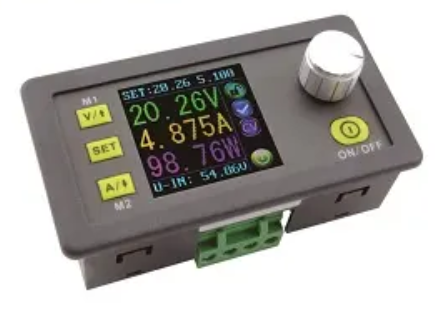
\includegraphics[width=\linewidth]{dcdc.png}
		\caption{DPS5005 50V 5A DC-DC Adjustable Buck Converter}
		\label{fig:dcdc}
	\end{figure}
	
	An AC-DC converter can be either linear or switching, a basic linear AC-DC converter is consisted of a transformer and a rectifier. The transformer can be laminated or toroidal, laminated transformers are cheaper, but toroidal transformers provide more power with a lower size and less external magnetic fields. Linear AC-DC converters are generally heavier and less efficient, but they are more cost-effective and provide a low noise output. A switching AC-DC converter is basically a rectifier and a DC-DC switching converter, that's why it is possible to integrate the AC-DC and DC-DC converters when they are both switching ones. Switching power supplies are efficient(less cooling), light, compact and more durable, but generally more complex and noisy. Switching action creates a lot of noise and ripple that is quite hard to eliminate, the spikes created by switching demand shielding, filtering and thus a more complicated PCB.

\section{Adjustable DC-DC converter}
	After we've made a clean and static DC voltage from the mains voltage, it is time to make current and voltage adaptable to user's will. For that we would need adjustable current and voltage regulators, they can be switching, linear or a combination of both. Switching regulators are a lot more efficient but more complicated, expensive and noisy, they can have various topologies such as boost, buck, buck-boost, flyback, or forward converters. One of the advantages of switching regulators is that they can boost the voltage up, which would be helpful when the AC-DC converter is provided by the user, and it has a low voltage. 

	Linear regulators on the other hand are simple, cheap, fast, and they don't introduce any noise to our circuit, however when the voltage drop across the regulating transistor goes up the power loss increases and can result in plenty of excess heat therefore it would require large heat sinks and fans. In completely linear bench power supplies, transformers have multiple terminals to produce different levels of voltages, and the regulator would be able to use the lowest one to avoid further losses.
	
	There is also another option where we can combine the best of both worlds, switching regulators can be used before linear regulators (Switchmode pre-regulator) to drop the voltage down and boost the efficiency of the regulating transistor, thus keeping the advantages of the linear regulator and omitting the disadvantage by boosting efficiency. It hasn't been done before, but in theory we could make the switchmode pre-regulator optional and modular, where the user would be able to later add it as an additional module or even remove it when needed.
\section{Control and monitoring circuitry}
    A bench power supply is never complete without a user interface, displaying and adjusting the output voltage and current is the bare minimum of functionality. To convert user input to what our circuits need we have two options, one is to use potentiometers and divide a known voltage, so it will be fed into the adjustable regulators and set the desired output, this method is very cost-effective, and we can easily increase the accuracy by using potentiometers in series.

	The other method is usually used in higher end products and requires a rotary encoder to capture user's input and then process it and pass it to a DAC or a PWM generator that would supply a DC voltage into the regulators to adjust the output, this way we would be able to program our power supply, but precision becomes expensive.
	
	There is also needs for temperature monitoring and digital means to shut off the output when something goes wrong. A micro-controller is inevitable, STM32 series can have a low price and are pretty versatile, choosing the exact model would require further tests and experiments.
	
	The display can be off the shelf seven-segments, seven-segments built on the PCB or character LCDs, it is said that seven-segments built with LEDs on the PCB are cheaper, but we have to confirm that with further research.
		
\section{Protection circuitry}
	We would have to add protection mechanisms after the primary design of the circuits is complete.
\section{Main chassis}
	This needs further research as to chose what kind of chassis is cheaper to use or more suitable for cooling and EMI. Generally the chassis should be easily seperatable from the front panel or the AC-DC converter as these parts should have the ability to be sold separately or in a package for users to assemble(Figure \ref{fig:case}).
	\begin{figure}
		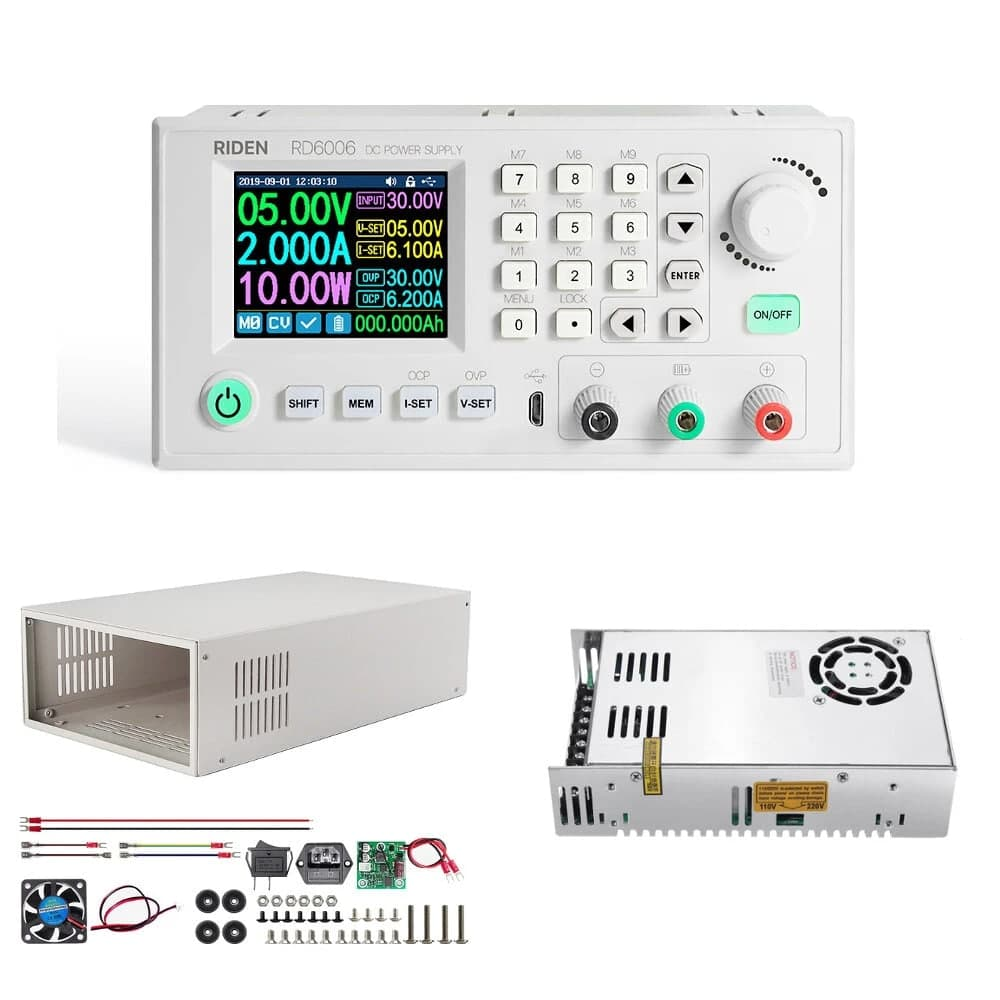
\includegraphics[width=\linewidth]{case.jpg}
		\caption{RD6006 60V 6A DC-DC Adjustable Buck Converter}
		\label{fig:case}
	\end{figure}
	
\section{Front panel}
	Front-panel can be plexiglass or molded plastic, but with the modularity and mounting mechanisms we would need molded plastic, although the exact method and materials need further research. The front panel is quite tricky to design, we would have to match the height of the components such as knobs, buttons or LEDs as the PCB would be holding them against the front panel. 
\section{Cooling}
	Cooling can be quite expensive, fans and big heat-sinks offer good thermal performance, but they can quickly drive the costs up. To counter this, we would have to use everything we have to cool the power transistors as much as possible, such as mounting them to the metal chassis or using the PCB as a heat-sink.

\section*{Compatibility}
	The end product has to be compatible with different use-cases either by accessories or by default to attract as many customers as possible. Electrophoresis can be done with voltages below 50 volts too, we could make electrophoresis modules and sell as accessories, phone repair services use bench power supplies, we could make banana plug to USB converters which use a small PCB and sell it as accessories. Medical electronics usually go through human safety standards, and being compatible with these standards can grow our customer base. Although, further research can discover even more use-cases which we could advertise and adapt our product to it.

\section*{Conclusion}
	Alright! We will be making a modular bench power supply where the main module is integrated into the front panel and the chassis along with the AC-DC converter are sold separately or pre-assembled, moreover there would be an optional switchmode pre-regulator which would be a piece of PCB where the user can purchase and install it to get more current output.
\section*{What To Do}
	\begin{enumerate}
		\item The plugin mechanism for the front panel and the PCB modules should get sorted out.
		\item Concurrent voltage and current regulation mechanisms should be designed and tested.
		\item A switchmode pre-regulator needs to be designed.
		\item Microcontroller code and circuitry needs to be designed.
		\item AC-DC converter's design should start.
		\item Research on protection circuits can begin now.
		\item Decisions on production methods, and materials for the front panel and the main chassis should be made.
		
	\end{enumerate}

	
	
\section*{Future Plans}
	\begin{enumerate}
	
		\item Primary design (make design decisions and design something that barely works)
	
		\item Improve the design (find and employ international standards and add fail safe mechanisms)
	
		\item Gather money and prototype the product
	
		\item Find investors
	
		\item Production design
	
		\item Website and shop
	
		\item Production run
	
		\item Advertisement \& product launch

	\end{enumerate}
\end{document}
